% --------------------------------------------------------------------

\section{Johdanto}

Tämä kandinaatintyö käsittelee eleentunnistusta Kinect-syvyyskameran avulla. 
Työn tarkoitus on tutustua erilaisiin eleentunnistusmenetelmiin ja erityisesti Chalearn Gesture Challenge -kilpailun kilpailutöihin. 
\\

Kuvaa ja videokuvaa on tutkittu paljon, mutta eleentunnistus on edelleen suuri haaste. Ihmisen eleet
ovat monimutkaisia ja niiden esitystapa vaihtelee esiintyjästä ja tilanteesta riippuen. Eleentunnistuksella
on kuitenkin monia käyttötarkoituksia esimerkiksi erilaisissa elekäyttöliittymissä. Toistaiseksi
eleentunnistusmenetelmät eivät ole olleet riittävän luotettavia ja nopeita, jotta niitä olisi voitu
laajasti hyödyntää kuluttajasovelluksissa.\\

Kehittynyt tekniikka kuten Microsoftin Kinect-sensori ja kehittynyt laskentateho tuovat alalle uusia mahdollisuuksia. 
Kinect-sensori on Microsoftin kehittämä 3D-kamera, joka tarjoaa 3D-videokuvaa eli tavallisen värikuvan 
lisäksi Kinect-kamera antaa infrapunakameralla mitattua syvyyskuvaa. 
3D-videokuvan avulla eleitä voidaan tunnistaa 2D-videokuvaa luotettavammin. 3D-kuva ei ole kuitenkaan 
vielä toistaiseksi radikaalisti kehittänyt tai muuttanut olemassa olevia eleentunnistusmenetelmiä.\\

Lisätäkseen kiinnostusta 3D-kuvaan järjestettiin ChaLearn Gesture Challenge -eleentunnistuskilpailu, 
jossa kilpailijat kehittivät Kinect-sensorin datalle suunnattuja 
eleentunnistusmenetelmiä. Tämä kandinaatintyö tutustuu kilpailutöihin ja kartoittaa niiden avulla alan uusinta tutkimusta. Kilpailu on hyvä tutkimuskohde,
sillä sen avulla voidaan puolueettomasti vertailla erilaisia menetelmiä. Eleentunnistukselle on tyypillistä, 
että menetelmät oppivat liiankin hyvin opetusdatajoukkoon, eivätkä ole enää yleistettävissä muille datajoukoille.
Jotta saadaan vertailtavissa olevia tuloksia, on eri menetelmiä testattava samalla ja mielellään kokonaan uudella datajoukolla.\\

ChaLearn Gesture Challenge -kilpailussa jaettiin Kinect-sensorilla kuvattuja näytteitä erilaisista eleistä.
Jokaisesta eleestä annettiin yksi näyte, koska kilpailijoita haluttiin kannustaa kehittämään yhdestä 
eleestä oppimiseen sopivia menetelmiä (One Shot Learning). Kilpailutöiden menetelmät olivat pääasiallisesti sellaisia,
että ne soveltuisivat myös tavalliselle 2D-videokuvalle. Menetelmät yhdistelivät tunnettuja menetelmiä kuvan-, videon- ja äänentunnistuksesta.\\

Luvussa kaksi esitellään tarkemmin eleentunnistusongelmaa ja 3D-videokuvaa. Luvussa kolme kerrotaan
ChaLearn Gesture Challenge -kilpailusta ja luodaan yleiskatsaus kilpailutöihin. Luvussa neljä esitellään
tarkemmin kolme kilpailutöistä.\\

Työ pyrkii kartoittamaan minkälaisia keinoja 3D-videokuvan tunnistuksessa voidaan käyttää ja mitä uutta 3D-kuva tuo verrattuna 2D-kuvaan.
Työssä esitellään jonkin verran hahmontunnistuksen käsitteitä ja käytäntöjä, mutta pääasiallisesti lukijan oletetaan tuntevan hahmontunnistuksen 
peruskäsitteet. Työ ei ota kantaa menetelmien tekniseen toteutukseen, vaan keskittyy teorian kuvaamiseen. Työssä ei myöskään keskitytä Kinect-kameran
teknisiin ominaisuukseen, vaan kameraa esitellään ainoastaan ongelman ymmärtämisen kannalta välttämätön määrä.


\section{Eleentunnistus videokuvalta}
\label{eleentunnistus videokuvalta}


\subsection{Eleentunnistus ongelmana}
Eleentunnistuksella tarkoitetaan tässä työssä ihmisen suorittaman eleen tunnistamista videokuvalta. Eleitä voisivat olla esimerkiksi
viittomakielen eleet tai yksinkertaiset toiminnot kuten istuminen. Eleentunnistus on haastava ongelma. Ihmisen eleet ovat
monimutkaisia ja videokuvalla on paljon muuttujia kuten valaistus, tila tai kohteen etäisyys kamerasta \citep {1251144}. 
Luokan sisällä on paljon vaihtelua eli sama ele näyttää erilaiselta videonäytteestä riippuen.
Yhtenä haasteena on ollutkin riittävän monipuolisen opetus- ja testitietokannan kerääminen.
\citep{4587756} Microsoftin Kinect-sensorin tapaisten syvyyskameroiden avulla haasteisiin voidaan kuitenkin vastata entistä tehokkaammin \citep {6239178}.\\

Eleentunnistus on hyvä erottaa asennontunnistus(Pose Estimation)-ongelmasta.
Asennontunnistuksessa pyritään tunnistamaan ihmisen asento videolla yhdessä pysäytyskuvassa
käyttämättä lainkaan ajallista tietoa. Tunnistuksessa pyritään usein tunnistamaan ihmishahmon ruumiinosat esimerkiksi nivelet,
joiden pohjalta arvioidaan asento. Ongelmana asennontunnistus on tietyssä mielessä helpompi
kuin eleentunnistus, sillä hahmontunnistus kuvalta on yksinkertaisempaa kuin videokuvalta ja sitä on tutkittu enemmän. 
Yksittäisiä asentoja voidaan käyttää tunnistamaan kokonainen ele, joskin se on laskennallisesti raskasta. \citep{5995316}  \\

Kiinnostus eleentunnistusta kohtaan on lisääntynyt viime vuosina sen monien käyttötarkoitusten vuoksi.
Eleentunnistusta voidaan käyttää monenlaisissa elekäyttöliittymissä.  Yksittäisiä eleitä voidaan 
käyttää esimerkiksi kodinkoneiden ohjailuun. \citep {1251144} Toisaalta eleentunnistusta voidaan käyttää hyödyksi tunnistamaan
erilaisia vaaratilanteita. Esimerkiksi potilaan tilaa voidaan seurata eleentunnistuskameralla 
mahdollisten poikkeavien eleiden varalta.\citep{chalearn2}\\

Videokuvan tunnistuksessa voidaan hyödyntää perinteisiä hahmontunnistusmenetelmiä. Monet menetelmistä ovat kuitenkin laskennallisesti liian raskaita 
reaaliaikaiseen videokuvan tunnistukseen, jota vaaditaan elekäyttöliittymissä. \citep {1251144}
Monet hahmontunnistusmenetelmät vaativat myös paljon opetusdataa. Kuluttajille suunnatuissa
sovelluksissa olisi toivottavaa, että uuden eleen voi opettaa muutaman testinäytteen perusteella \citep {1251144}.
Eleentunnistusmenetelmien on kyettävä vastaavaan näihin haasteisiin.\\

Eleentunnistuksessa, kuten hahmontunnistuksessa yleensä, korkeimpana tavoitteena on jäljitellä ihmisen toimintamalleja.
Ihmisen kyky tunnistaa ja oppia hahmoja on erinomainen. Ihminen kykenee oppimaan eleet yhden opetusnäytteen perusteella 
ja tunnistaa eleet tehokkaasti ulkoisista muuttujista riippumatta. Käytännössä huimaa vauhtia kehittynyt tekniikka on kuitenkin
viime aikoina ajanut tutkimuksen ohi ja monet menetelmät on kehitetty nopeasti lähinnä vastaamaan käytännön tarpeisiin. Samalla 
ihmisen jäljittely -näkökulma on unohdettu.
\citep{chalearn2}

\subsection{3D-videokuva}
Kinect-sensori on Microsoftin kehittämä kaupallinen 3D-kamera. Se on tarkoitettu Microsoftin Xbox-pelikonsolin lisäosaksi.
Kamera kehitettiin ensisijaisesti viihdekäyttöön parantamaan Xbox-pelien käyttökokemusta. Microsoft on kuitenkin avannut
Kinectille ohjelmointirajapintoja, joiden avulla Kinect-kameralle on kehitetty lukuisia alkuperäisestä käyttötarkoituksesta 
irrallisia sovelluksia.\citep{kinect}\\

Tavallisen värikuvan lisäksi Kinect-sensori tarjoaa syvyyskuvaa kohteesta. Syvyyskuva kertoo kohteen etäisyyden kamerasta ja luo näin kolmiulotteista videokuvaa. 
Microsoft tarjoaa Kinectille myös ohjelmistokehitystyökaluja, jotka sisältävät erilaisia hahmontunnistustyökaluja.
Niiden avulla kehittäjä saa käyttöönsä esimerkiksi ranganseurauksen eli tiedon ihmishahmon asennoista videokuvan eri hetkillä. \citep{kinect}\\
Myöhemmin esiteltävässä ChaLearn Gesture Challenge -kilpailussa kilpailijat eivät kuitenkaan hyödyntäneet Microsoftin tarjoamia 
valmiita hahmontunnistustyökaluja, vaan kilpailun tarkoitus oli kehittää omia menetelmiä. \\

Eleentunnistuksen näkökulmasta syvyyskuvalla on monia etuja verrattuna värikuvaan. Syvyyskuva on yksiväristä
eli siitä on riisuttu erilaiset värit ja tekstuurit, jotka usein aiheuttavat ongelmia värikuvan tunnistamisessa.
Syvyyskuvan värisävyt on pakotettu tietylle asteikolle, mikä helpottaa kuvien vertailtavuutta. \citep{5995316} Hahmo on helposti erotettavissa
taustastaan ja eleet, jotka eroavat toisistaan ainoastaan syvyyssuuntaisen liikkeen perusteella, 
on mahdollista erottaa huomattavasti luotettavammin kuin pelkän värikuvan perusteella.\\
 
Kuvassa ~\ref{fig:kinectkuva} on esimerkki Kinectin värikuvasta ja syvyyskuvasta. Kuvat ovat samasta tilanteesta.
Syvyyskuvasta näkee hyvin syvyyskameran hyödyt. Hahmo on helposti erotettavissa taustasta ja hahmon käsi, 
joka on vartalon edessä voidaan helposti erottaa omaksi raajakseen. \\

\begin{figure}[htb]
  \begin{center}
    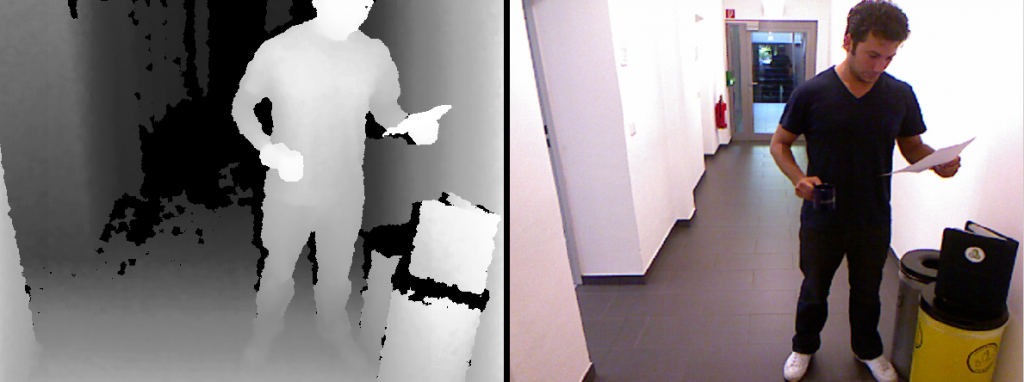
\includegraphics[width=0.9\textwidth]{kinect1_cropped-1024x382.png}
    \caption{Esimerkki Kinectin syvyyskuvasta (vasemmalla) ja värikuvasta (oikealla). \citep {kinectkuva}}
    \label{fig:kinectkuva}
  \end{center}
\end{figure}

\subsection{Eleentunnistus video- ja 3D-videokuvalta}

Eleentunnistus videokuvalta noudattaa tavallisia hahmontunnistuksen vaiheita: esikäsittely, piirrevalinta ja
luokittelu. Eleentunnistuksen erityishaasteet on huomioitava erityisesti piirrevalinnassa. 3D-videokuva tuo 
oman lisänsä, mutta se ei merkittävästi muuta työvaiheita. Eleentunnistus on hahmontunnistuksen termein
luokitusongelma eli mahdolliset luokat tunnetaan ennalta. \citep{6239178}  \\

Esikäsittelyvaiheessa videokuvalta poistetaan häiriötä, jotka voisivat haitata eleentunnistusta.
Näitä voivat olla esimerkiksi kuvassa esiintyvät ylimääräiset objektit tai videokuvan virheet kuten kohina.
Kuvaa voidaan myös pienentää tai pakata laskennan nopeuttamiseksi. Esikäsittelyssä pyritään usein myös erottamaan ihmishahmo taustasta. Tämä on haastavaa, sillä
ihmishahmo ei välttämättä erotu esimerkiksi väritykseltään taustasta. Kinectin syvyyskameran avulla taustan irrotus onnistuu kuitenkin luotettavammin kuin pelkän 
värikuvan avulla. Ihmishahmon erottaminen taustasta helpottaa tunnistusta, sillä tällöin ihminen ei sekoitu taustaansa tai mitään taustassa olevaa
esinettä ei erehdytä pitämään ihmisen osana. Esikäsittelyssä voidaan suorittaa myös jonkinlaista ajallista jakoa tai tiivistystä. Videokuvaa
voidaan esimerkiksi jakaa ajallisiin jaksoihin perustuen videokuvan samankaltaisuuteen. Ajallisen jaon 
tarkoitus on auttaa hahmottamaan kuvalla tapahtuvaa liikesarjaa ja helpottaa tunnistusta.\citep{6239178} \\

Hahmontunnistuksessa ratkaiseva vaihe on usein oikeiden piirteiden valinta eli piirreirrotus. Videokuvasta voidaan valita piirteeksi esimerkiksi 
tietyn suuntainen liike ajan funktiona. Liike näkyy peräkkäisten pysäytyskuvien välisenä erona. Tutkimalla liikettä
videokuvat voidaan tiivistää liikekuviin, joita voidaan luokitella yksinkertaisilla luokittelualgoritmeillä. 
Videokuvaa voidaan tarkastella myös yksittäisten pysäytyskuvien kautta. 
Tällöin voidaan hyödyntää valokuvien tunnistuksessa käytettyjä menetelmiä.
Pysäytyskuvista voidaan arvioida kontrastivaihteluita ja sitä kautta hahmottaa viivoja tai muotoja kuvassa. \citep{6239178}  \\

Tunnistusvaiheessa näytteitä verrataan opetusdatan kuvaamiin luokkiin. Tunnistusmenetelmä riippuu valituista piirteistä.
Jos videokuvaa käsitellään kokonaisuutena esimerkiksi liikekuvan avulla, kuvia voidaan luokitella yksinkertaisilla luokittelualgoritmeillä. 
Näitä voisivat olla esimerkiksi k-lähimmän naapurin luokitin. Jos videokuva esitetään yksittäisillä pysäytyskuvilla 
on tunnistuksessa huomioitava videon aikaulottuvuus. On käytettävä rakenteellista mallia, jonka avulla voidaan tarkastella piirteen arvoa
tietyllä ajanhetkellä. Tähän tarkoitukseen on erilaisia graafisia malleja, joita esitellään tarkemmin luvussa kolme. \citep{6239178} \\

Luokittelun jälkeen menetelmälle lasketaan virheprosentti. Virheprosentti lasketaan testidatan avulla.
Testidatassa on opetusdatan tavoin annettu näytteiden oikeat luokat, jolloin on mahdollista laskea, kuinka suuri prosentti
näytteistä on luokiteltu oikeisiin luokkiin. Menetelmää voidaan kehittää edelleen kokeilemalla erilaisia
opetusdatajoukkoja ja valitsemalla joukko, joka tuottaa pienimmän virheprosentin testidatalle. \citep{6239178} 

\section{ChaLearn Gesture Challenge -kilpailu}
\label{ChaLearn Gesture Challenge -kilpailu}

\subsection{Kilpailun esittely}
ChaLearn Gesture Challenge -kilpailun tarkoituksena oli lisätä kiinnostusta eletunnistukseen syvyyskameralla.
Kilpailu alkoi vuoden 2011 lopuilla ja se päättyi loppuvuonna 2012. Kilpailuun osallistui ensimmäisellä kierroksella 50 ryhmää,
pääasiallisesti yliopistojen tutkimusryhmiä. Kinect-sensorin kehittäjä Microsoft lahjoitti palkinnot kilpailuun.
Kilpailussa tarjottiin tietokanta, joka sisälsi 50 000 Kinect-sensorilla kuvattua videonäytettä. Videonäytteet sisälsivät yksittäisiä
eleitä, esimerkiksi viittomia tai poliisin käsimerkkejä. Kilpailijoiden tarkoitus oli kehittää eleentunnistusmenetelmä, jonka avulla eleet
opitaan yhdestä opetusnäytteestä. Eleitä oli jaettu kategorioihin käyttötilanteen mukaan. Esimerkiksi poliisin käsimerkit olivat yksi kategoria.
\citep{6239178} \\

Annetuilla videonäytteillä esiintyi aina yksi ihminen kerrallaan suorittamassa tiettyä elettä. Kuva rajattiin yläruumiiseen ja eleet tehtiin
pääasiallisesti käsillä. Liikkeet lopetettiin ja aloitettiin aina samasta lepoasennosta. Videonäytteet sisälsivät syvyyskamerakuvan sekä värikuvan, 
mutta eivät ranganseurausta tai muuta valmista hahmontunnis tietoa. Haasteita toivat vaihtelevat taustat ja valaistukset videokuvalla.  \citep{6239178}\\

Kilpailijoille jaettiin kolme datajoukkoa: opetusdata, validointidata ja lopullinen arviointidata. 
Opetusdatan näytteille tarjottiin oikeat luokat, joiden avulla järjestelmän opetus onnistui.
Sekä validointidatassa, että lopullisessa arviointidatassa jokaisesta eleestä annettiin ainoastaan yksi opetusnäyte eli näyte,
jolle oli paljastettu oikea luokka. Kilpailun erityishaasteena olikin yhdestä otoksesta oppiminen (One Shot -learning). 
Tarkoituksena oli kehittää järjestelmä, joka oppii tunnistamaan eleet mahdollisimman pienestä määrästä opetusdataa. 
Kilpailijoiden odotettiin soveltavan tässä siirtovaikutusoppimista (Transfer learning). \citep{6239178} \\

Siirtovaikutuksen ajatus on, että aiemmin opittuja tietoja hyödynnetään seuraavassa oppimistehtävässä. Tässä jäljitellään  
ihmisen oppimiskykyä. Ihminen oppii nopeasti tunnistamaan uusia hahmoja, jos hänellä on kokemusta vastaavista tehtävistä.
Siirtovaikutuksessa tietoja siirretään edellisestä oppimisprosessista uuteen oppimistehtävään.
Siirretyt tiedot saattavat olla esimerkiksi aiemmassa opetustehtävässä valitut piirteet tai jopa yksittäisiä datanäytteitä. \citep{5288526}\\

Järjestelmä, jonka avulla kilpailijat pystyivät testaamaan menetelmäänsä validointidataa vastaan, oli auki koko kehitysjakson ajan.
Varsinainen testidata, joilla kilpailutöitä arvosteltiin paljastettiin vasta kilpailun lopuksi. Kilpailijoilla oli muutama päivä aika
testata menetelmäänsä lopullista testidataa vastaan. Testidata sisälsi eri eleitä kuin opetusdata, mutta samoista kategorioista.
Kilpailijoiden oli siis opetettava menetelmänsä uudelleen lopullisen testidatan avulla. Kilpailijoita pyydettiin lopuksi
palauttamaan lista, joka sisälsi oikeat luokat testidatalle esitettynä merkkijonona. Lopullinen virheprosentti saatiin laskemalla Levensteinin etäisyys
oikeita luokkia kuvaavan merkkijonon ja kilpailijoiden antaman vastausmerkkijonon välillä. \citep{6239178} 


\subsection{Katsaus kilpailutöihin}
\subsubsection {Ensimmäinen kierros}
Kilpailijoiden metodeja selvitettiin ensimmäisen kierroksen jälkeen lyhyellä kyselyllä, johon vastasi 20 ryhmää 22 parhaan ryhmän joukosta.
Ryhmiltä kysyttiin muun muassa minkälaista esikäsittelyä he olivat tehneet videokuvalle, minkälaista tunnistusmenetelmää tai mitä piirteitä oli käytetty ja
mikä oli heidän menetelmänsä suoritusaika. Kyselyn tarkoituksena oli saada yleiskatsaus kilpailutöihin, sillä monet kilpailijat eivät
halunneet julkaista yksityiskohtaista kuvausta menetelmästään kilpailun ollessa vielä kesken. \citep {6239178}. \\

Vastauksista kävi ilmi, että lähes kaikki ryhmät tekivät jonkinlaista kuvan esikäsittelyä. Videokuvasta poistettiin häiriötä, asiaankuulumattomia 
kohteita tai ihmishahmon tausta. Huomioitavaa on kuitenkin, että jotkin hyvin menestyneistä ryhmistä eivät tehneet minkäänlaista esikäsittelyä kuvalle.
\citep {6239178}\\

Suurin osa osallistujista käytti piirteinä HOG/HOF-piirteitä (Histogram of oriented Gradients/ Histogram of Flow), SIFT/STIP-piirteitä 
(Scale Invariant Feature Transformation/Space-time interest points), 
kulmien tai nurkkien tunnistusta tai kehitti omia, tälle datalle soveltuvia piirteitä.\citep {6239178}\\

Käytetyt piirteet perustuvat pääosin kuvan värityksen intensiteettivaihteluun.
Esimerkiksi HOG-piirteet kuvaavat kuvan intensiteettivaihtelun gradienttien suuntaa. Kuva jaetaan pieniin alueisiin, soluihin, 
joissa tarkastellaan alueen värityksen intensiteettivaihtelua. Soluille lasketaan intensiteettivaihtelun gradienttien suuntien histogrammi. 
Ajatuksena on päätellä, minkä suuntaisia viivoja tai nurkkia alueelta voidaan erottaa.\citep {1467360} Histogrammit kertovat kuvassa esiintyvistä
muodoista, eivätkä ne ole riippuvaisia hahmon sijainnista kuvassa tai kuvan yleisestä värimaailmasta.
HOG-piirteet soveltuvatkin hyvin tämänkaltaiseen hahmontunnistusongelmaan, jossa kohteen sijainti ja väritys voivat vaihdella kuvalla.
HOF-piirteet toimivat samoin kuin HOG-piirteet, paitsi kuvien sijaan ne tutkivat liikettä, optista virtaa, videolla \citep{Pers20101369}.\\

SIFT-piirteet toimivat HOG-piirteitä hienostuneemmin valiten kuvista tärkeät pisteet. Tärkeät pisteet valitaan niin, että ne ovat riippumattomia
kuvan muutoksista kuten kiertämisestä tai skaalauksesta. Esimerkiksi kuvassa, jossa näkyy ovi, tärkeitä pisteitä voisivat olla oven kulmat.
Vaikka kuvaa kierrettäisiin tai sen kokoa muutettaisiin, tärkeät pisteet eli kulmat voidaan löytää kuvasta.
Pisteiden valinnassa hyödynnetään värityksen intensiteettivaihtelua ja tilastollisia menetelmiä.  \citep {790410}
STIP-piirteet perustuvat samankaltaiseen menetelmään \citep{1238378}. \\

Piirteitä voidaan tutkia syvyys- ja värikuvasta. Syvyyskuvan etu verrattuna värikuvaan on, että siinä
ei esiinny värejä tai tekstuureja, jotka häiritsisivät hahmon erottumista tai videoiden vertailua.
Suurin osa kilpailijoista käyttikin töissään pelkkää syvyyskuvaa. Osa käytti sekä väri- että syvyyskuvaa. 
Mielenkiintoista on, että ensimmäisen kierroksen toisen sijan voittaja käytti työssään pelkkää värikuvaa. 
Kaikki kilpailijat käyttivät jonkinlaista piirteiden tiivistystä tai kuvausta toiseen lineaariavaruuteen. \citep {6239178}\\ 

Ajallisen rakenteen mallintamiseen käytettiin erilaisia graafisia malleja kuten Markovin piilomuuttujaa ja Conditional Random Fields -menetelmää.
Kaikki tunnistustusmenetelmät eivät kuitenkaan huomioineet videon ajallista rakennetta. \citep {6239178}\\ 

Markovin muuttuja kuvaa havainnon sarjana tiloja eli tässä tapauksessa videon sarjana pysäytyskuvia. 
Tilat esitetään sopivien piirteiden avulla eli esimerkiksi kuvat voidaan esittää HOG/HOF-piirteiden avulla. 
Menetelmä kertoo kuinka todennäköisesti annettu havainto kuuluu tiettyyn luokkaan. 
Ajatuksena on, että annetun havainnon luokka on tuntematon, mutta se voidaan löytää sen etsimällä todennäköisin luokka. 
Luokat saadaan opetusdatasta.\\

Luokkien tiheysfunktiot lasketaan suurimman todennäköisyyden
(Most Likelihood) -menetelmällä. Kyseessä on Bayesilainen menetelmä eli jakauma tunnetaan, mutta ei parametreja.
Parametrien arvot optimoidaan niin, että todennäköisyys opetusliikkeelle kuulua kuvaamaansa luokkaan on mahdollisimman suuri.
Luokan tiheysfunktion avulla voidaan laskea kuinka todennäköisesti tietty tilasarja esiintyy tässä luokassa.
Luokassa on kuitenkin useita mahdollisia tilasarjoja. Todennäköisyys annetulle havainnolle $O = O_{1}, O_{2}...O_{n}$ kuulua 
luokkaan $\lambda$ saadaan siis seuraavasti:
\begin{equation}
P(O,Q|\lambda) = \sum\limits_{all Q}P(O|Q, \lambda)P(Q|\lambda)
\end{equation}
jossa $Q = Q_{1}, Q_{2} ... Q_{n}$ eli Q on määrätyn mittainen tilasarja. Todennäköisyys havainnolle O esittää
tiettyä tilasarjaa Q kerrotaan todennäköisyydellä $P(Q|\lambda)$ eli todennäköisyydellä tilasarjalle Q esiintyyä luokassa $\lambda$. 
Lopuksi summataan yhteen todennäköisyydet sarjalle O kuulua luokkaan $\lambda$ kaikilla tilasarjoilla Q. 
Näin saadaan lopullinen todennäköisyys havainnolle O kuulua luokkaan $\lambda$. On huomioitava, että menetelmä vaatii
kaikkien näytteiden olevan samanpituisia eli koostuvan tietystä ennalta määrätystä määrästä tiloja. Tämä saattaa asettaa
rajoituksia menetelmän sovelluksissa.\citep {18626}\\

Conditional Random Fields -menetelmä perustuu samankaltaiseen intuitioon. \citep {1315232} Lähtökohta molemmissa on, että yksittäisen 
datapisteen sijaan luokitellaan datajoukkoja, joilla on sisäinen, tässä ajallinen, rakenne. Kilpailutöissä, joissa ei käytetty 
ajallisen rakenteen mallintamista, luokittelussa käytettiin k-lähimmän naapurin luokitinta tai muita yksinkertaisia luokittelumenetelmiä. \\

Kilpailun järjestäjien odottamaa metodia, siirtovaikutusta käytettiin vähäisesti, eikä kukaan menestyneistä kilpailijoista käyttänyt sitä.
Kilpailun varsinainen haaste, yhdestä eleestä oppiminen, jäi siis vähemmälle huomiolle. \citep {6239178} \\

Kahdeksan menestyneintä työtä esitellään taulukossa ~\ref{table:dvbt_param}. Taulukosta huomataan, että parhaiten menestyneiden töiden
joukossa suurin osa käytti tunnistuksesa menetelmää, joka huomioi videon ajallisen rakenteen. Tällöin videokuvasta valitaan piirteet, joiden
muutosta seurataan ajan funktiona. Poikkeuksen tekevät ryhmät Zonga ja Xiaozhuwudi, joiden menetelmä perustuu videon käsittelyyn erilaisten liikekuvien avulla. 
\citep {6239178}\\

\begin{table}[th]
\caption{ChaLearn Gesture Challenge -kilpailun kahdeksan parhaiten sijoittunutta ryhmää}
\label{table:dvbt_param}
\begin{center}
\begin{tabular}{|p{0.35\textwidth}|p{0.45\textwidth}|} 
    \hline
Ryhmän nimi & Menetelmä \\
    \hline
    \hline
Alfnie & Motion Signature analyses\\ 
    \hline
Pennect & Markovin piilomallin tapainen menetelmä ja HOG/HOF-piirteet.\\
    \hline
One Million Monkeys & Markovin piilomalli ja kulmien tunnisus\\
    \hline
Immortals & Markovin piilomalli ja HOG/HOF-piirteet\\
    \hline
Zonga & Pienimmänneliösumman menetelmä ja HOSVD -menetelmä\\
    \hline
Balazs Godeny & Thumbnail Dynamic Time Warping” (DTW) ja HOG/HOF-piirteet sekä kulmien tunnistus.\\
    \hline
SkyNet & Dynamic Time Warping(DTW) ja kulmien tunnistus\\
    \hline
Xiaozhuwudi & MHI-kuva johon on lisätty GEI- ja INV-kuvat\\
    \hline	
\end{tabular}
\end{center}
\end{table}

Luvussa neljä esitellään kolme menestyneistä töistä tarkemmin. Työt ovat eräitä esimerkkejä toimivista ratkaisuista. Ne on valittu tähän, 
koska ne edustavat erilaisia näkökulmia ongelmaan. Valintamahdollisuuksia rajoitti se, että kaikki kilpailijat eivät olleet vielä julkaisseet 
menetelmäänsä tämä työn kirjoittamisen aikana. Kolmesta valitusta työstä yksi, Immortals edustaa kilpailun yleislinjaa ja kaksi muuta valittua työtä,
Zonga ja Xiaozhuwudi ovat esimerkkeinä omaperäisemmistä menetelmistä.\\

\subsubsection {Toinen kierros}

Kilpailun toinen kierros toteutettiin samoilla järjestelyillä kuin ensimmäinen. Koska kierros loppui
vasta tämän kandinaatintyön kirjoittamisen aikoihin, on se jätetty työssä vähemmälle tarkastelulle.\\

Toisen kierroksen jälkeen kilpailijoiden metodeja selvitettiin kyselyllä samoin kuin ensimmäisen
kierroksen jälkeen. Kyselyyn vastasi 28 ryhmää. Vastausten perusteella toisella kierroksella menestyneet 
menetelmät olivat hyvin samantapaisia kuin ensimmäisen kierroksen menestyneet menetelmät. HOG/HOG-piirteet sekä muut
kuvan intensiteettivaihteluihin perustuvat piirteet yhdistettynä Markovin piilomuuttujaan tai muuhun
vastaavaan malliin olivat suosituin menetelmä. \citep{chalearn2}\\

Molemmilla kierroksilla oli sama voittaja, ryhmä Alfnie. 
Voittajaryhmä väittää työnsä matkivan ihmisen hahmontunnistuskykyä. Työtä ei ole kuitenkaan vielä tämän kandinaatintyön kirjoittamisen aikaan julkaistu,
 joten siihen ei päästä tutustumaan tarkemmin. Työ perustuu
ryhmän ilmoituksen mukaan jonkinlaiseen mukautettuun Markovin piilomuuttujaan. Mielenkiintoista on,
että huolimatta hyvästä sijoituksestaan menetelmä oli myös yksi kilpailun nopeimmista. \citep{chalearn2}\\

Toisen sijan voittaja toisella kierroksella, ryhmä Turtle Tamers, käytti samankaltaista menetelmää kuin 
ensimmäisen kierroksen toisen sijan voittaja, ryhmä Pennect. Molemmat ryhmät käyttivät HOG/HOF-piirteitä sekä Markovin piilomuuttujaa. 
Kolmannen sijan saavuttanut ryhmä Joewan sen sijaan käytti hyvin erilaista menetelmää. Ryhmä käytti Bag of MOSIFT -
piirteitä yhdistettynä lähimmän naapurin luokittimeen. \citep{chalearn2} Bag of MOSIFT -piirteet on kustoimoitu versio
yleisestä Bag of features -menetelmästä. Bag of features -menetelmät kuvaavat tietyn piirteen avulla
kuinka usein tietty arvo esiintyy näytteessä. Ne mittaavat siis ainoastaan kuinka usein tietty arvo esiintyy näytteessä ja
hajottavat näin näytteen sisäisen rakenteen \citep{bagoffeatures}. \\

Varsinaisen validoinnin lisäksi kilpailutöille suoritettiin palautuksen jälkeen vielä yksi testaus. Tässä testauksessa tutkittiin kuinka 
hyvin kilpailijoiden menetelmät tunnistivat eleen, jos videokuvaa oli tietoisesti käännetty hieman. Oikeissa sovelluksissa on tärkeää,
että ele pystytään tunnistamaan, vaikka se eroaisi hieman alkuperäisestä näytteestä esimerkiksi kuvakulmaltaan. 
Tässäkin testissä voittajaryhmä pärjäsi hyvin, kun taas esimerkiksi kaksi seuraavaa ryhmää pärjäsit manipuloidulla datalla huomattavasti
huonommin kuin varsinaisella kilpailudatalla. Tämä lisää ennestään mielenkiintoa voittajatyötä kohtaan. \citep{chalearn2}


\section {Katsaus menestyneisiin kilpailutöihin}

\subsection{Xiaozhuwudi ja laajennettu MHI-menetelmä}
Ryhmä Xiaozhuwudi lähti liikkeelle MHI eli Motion History Image -menetelmästä \citep {6239179}. MHI tutkii liikkeen määrää videokuvalla.
Videopätkä tiivistetään yhteen liikekuvaan, joka kuvaa liikkeen viimeaikaisuutta. Kohdat, joissa videokuvalla on ollut
liikettä esitetään harmaasävyillä. Mitä viimeaikaisempaa liike on ollut sitä valkoisempana se näkyy kuvassa. Liikkumattomat
alueet näkyvät täysin mustana. Videokuvalta tutkitaan siis vain liikettä, eikä pyritä esimerkiksi tunnistamaan kuvalla olevia kohteita
tai ihmiskehon osia. Tämä menetelmä matkii ihmisen tapaa tunnistaa eleitä. Ihminen tunnistaa erittäin hyvin inhimilliset eleet  
sumealtakin videokuvalta vaikka ei yksittäisestä pysäytyskuvasta tunnistaisi edes ihmishahmoa. \citep {910878}  \\

\begin{figure}[htb]
  \begin{center}
    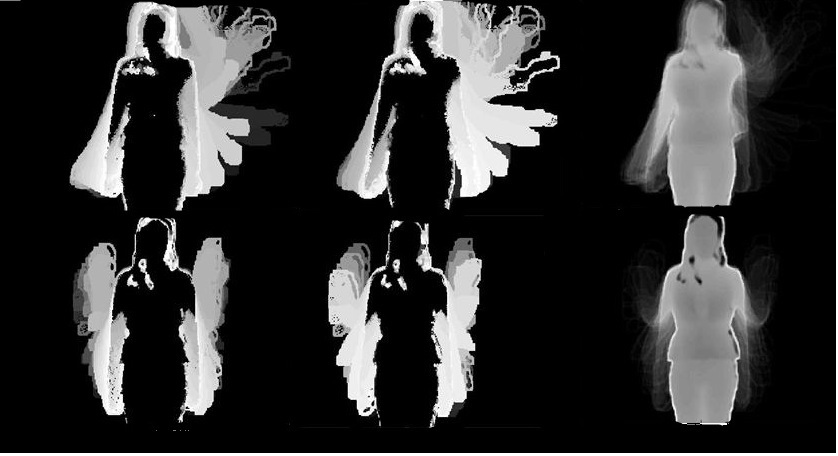
\includegraphics[width=0.9\textwidth]{mhi_ex.jpg}
    \caption{Kuvassa vasemmalta oikealle MHI, INV ja MEI. \citep {6239179}}
    \label{fig:mhiinvmei}
  \end{center}
\end{figure}

Xiaozhuwudi-ryhmä tunnistaa MHI-kuvassa kuitenkin ongelmia. MHI-kuvan avulla on vaikeaa tunnistaa eleitä, jotka sisältävät toistuvaa liikkeitä, esimerkiksi vilkutusta.
Liikkeen toistuessa MHI-kuva muuttuu helposti sekavaksi ja on vaikea erottaa tarkkaa liikerataa. Xiaozhuwudi ehdottaakin MHI-kuvan laajentamista 
INV(Inverse)- ja GEI(Gait Energy Image)-kuvilla. INV-kuva on MHI-kuvalle käänteinen kuva. INV-kuvassa katsotaan videokuvaa alusta loppuun päin.
Mitä aikaisemmin liike esiintyy videolla sitä vaaleampana se näytetään kuvassa. INV:n avulla saadaan kuvaus videon alkutilanteesta, mikä täydentää MHI kuvaa. 
GEI-kuva esittää liikkeen määrää keskimäärin koko videon aikana. Siinä summataan koko videon liike yhdelle kuvalle ja jaetaan lopuksi koko aikavälille.
GEI muistuttaa MEI:tä (Motion Energy Image), jossa myös lasketaan liikkeelle summa. Voidaan ajatella, että siinä missä MHI- ja INV-kuvat kuvaavat liikettä ,
MEI- ja GEI-kuvat mittaavat energiaa, joka on kulunut liikkeeseen. GEI-kuvan avulla liikkeestä saadaan hyvä kokonaiskuva ja se on hyödyllinen etenkin toistuvan
liikkeen tunnistuksessa. \citep {6239179} \\

Kuvassa ~\ref{fig:mhiinvmei} on esitetty kahdelle
liikkeelle MHI-, INV- ja GEI-kuvat. Kuvat havainnollistavat hyvin miten INV- ja GEI-kuvat
täydentävät MHI-kuvaa. Pelkän MHI-kuvan perusteella on vaikea erottaa liikkeet toisistaan.
INV- ja GEI-kuvien avulla liikkeet erottuvat kuitenkin selkeämmin. \\

Datan esikäsittelyssä Xiaozhuwudi hyödynsi Kinectin syvyyskuvaa poistamalla taustan ihmishahmolta. Lisäksi esikäsittelyssä poistettiin häiriöitä.
MHI, GEI ja INV -kuville suoritettiin dimensioiden vähennys. Eleiden tunnistukseen käytettiin Maximum Correlation Coeffient -luokittelijaa,
joka perustuu kuvien väliseen korrelaatioon. \citep {6239179}\\

Ryhmä väittää työnsä suoriutuvan eleentunnistusongelmasta huomattavasti nopeammin kuin muut paikalliseen tietoon perustuvat eleentunnistusmenetelmät.
Lisäksi menetelmä vastaa ryhmän mukaan paremmin yhdestä eleestä oppimisen -haasteeseen kuin esimerkiksi Markovin piilomuuttujaan perustuvat menetelmät.
\citep {6239179}

\subsection{Immortals ja Markovin piilomuuttuja}

Ryhmä Immortals esittää kilpailutyössään oletuksen, että ele koostuu ennen kaikkia useista yksittäisistä liikkeistä. 
Sen mukaan eleet tunnistetaan parhaiten käsittelemällä elettä sarjana liikkeitä. Tämä eroaa ryhmän mukaan tyypillisestä 
tavasta lähestyä ongelmaa.\citep {6239185}\\

Ryhmä lähti liikkeelle opetusvaiheessa yksittäisistä liikkeistä. Yksittäisille liikkeille luodaan allekirjoitus eli malli,
jonka avulla ne voidaan tunnistaa. Allekirjoituksen luominen on monivaiheinen operaatio. Ensin kuvista poimitaan niin sanotut
tärkeät pisteet eli pisteet joilla on merkitystä liikkeen tunnistamisen kannalta. Tässä Immortals hyödynsi Kinectin syvyyskuvaa.
Immortals arvioi, että ne kohdat kuvasta, joissa on tapahtunut syvyyssuuntaista muutosta syvyyskameran kuvassa ovat kyseisen videon pysäytyskuvan
tärkeitä pisteitä. Tärkeille pisteille lasketaan HOG(Histogram of Oriented Gradients)- ja HOF(Histogram of Flow)-histogrammit. 
Tämän jälkeen kaikkien kuvien kaikki histogrammit ryhmitellään tavallisen ryhmittelyalgoritmin avulla.
Histogrammeja kutsutaan ryhmittelyn jälkeen "visuaalisiksi sanoiksi". Yhdessä ryhmässä ovat kaikki tietyn sanan esiintymät.
Tarkoituksena on tutkia visuaalisten sanojen esiintymistä yhdessä ja muodostaa niistä aihepiirejä. 
Yksittäistä pysäytyskuvaa voidaan kuvata sillä, mitä sanoja ja mistä aihepiireistä siinä esiintyy.\citep {6239185}\\

Liikkeelle luodaan sanojen perusteella perusteella malli, jota käytetään tunnistusvaiheessa. Mallin perustana on Markovin muuttuja
eli HMM (Hidden Markov Model). Koska tutkitaan kahta piirrettä, HOG- ja HOF-piirrettä, käytetään monikanavaista Markovin piilomallia eli McHMM (Multi Channel Hidden Markov Model). 
HOG- ja HOF-piirteet paljastavat erilaista tietoa havainnosta ja tukevat tässä hyvin toisiaan. McHMM-mallin parametreja ovat alkutila, 
todennäköisyys tilojen väliselle siirtymälle sekä tilan todennäköisyys ja tilan kuvaus visuaalisten sanojen eli HOG- ja HOF-piirteiden avulla. 
Tilalla tarkoitetaan tässä yksittäistä pysäytyskuvaa. Malli opetetaan parametrien avulla niin, että se tunnistaa tietyn liikkeen eli tietyn
sarjan pysäytyskuvia.\citep {6239185} Kuvassa ~\ref{fig:HMM} on tarkennettu vielä Markovin piilomallin toimintaa. Kuvassa on 
esitetty havainto ja Markovin piilomuuttujan mahdolliset tilat, sekä niiden väliset siirtymätodennäköisyydet. Tarkoitus on löytää
tilasarja, joka todennäköisimmin on muodostanut tämän havainnon. Parametrit eli tilat ja todennäköisyydet on opetettu mallien perusteella. \\

\begin{figure}[htb]
  \begin{center}
    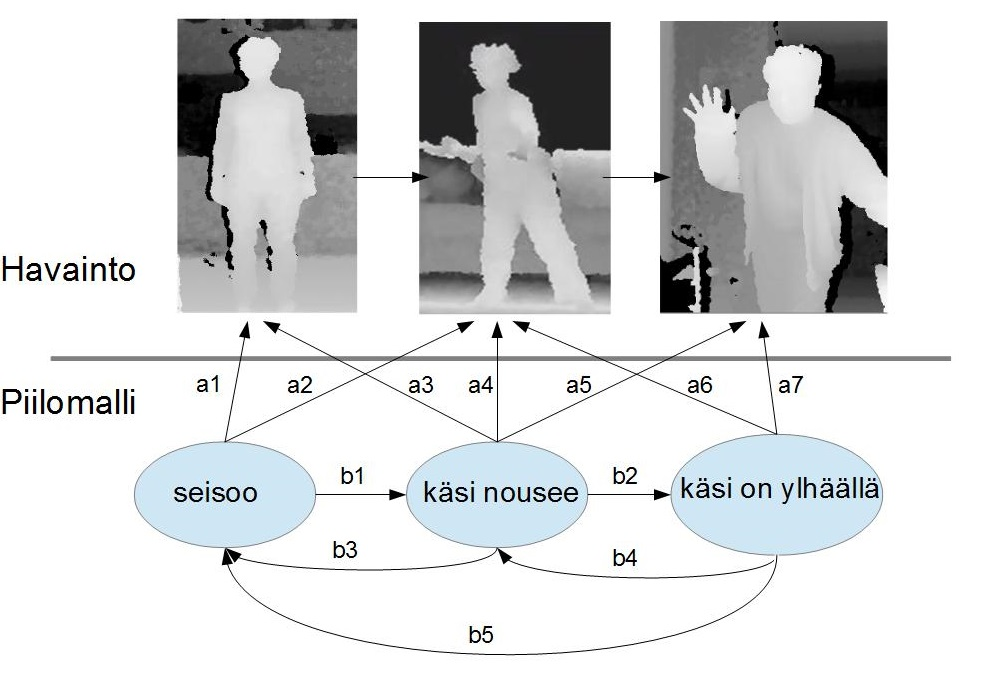
\includegraphics[width=0.9\textwidth]{HMModfcropped.jpg}
    \caption{Markovin piilomuuttujan käyttö eleentunnistuksessa. Viivan yläpuolella on havainto esitetty pysäystyskuvien avulla. Viivan alla ovat mahdolliset tilat,
	sekä niiden väliset siirtymätodennäköisyydet b1-bn. Todennäköisyydet a1-an kuvaavat kuinka todennäköisesti tila esittää havaittua tilaa.
	Tarkoituksena on löytää tilasarja, joka kaikkein todennäköisimmin muodostaa havainnon. Kuvan esittämässä tilanteessa todennäköisin tilasarja
	olisi varmaankin: seisoo, käsi nousee, käsi on ylhäällä.}
    \label{fig:HMM}
  \end{center}
\end{figure}

Tunnistusongelma pelkistyy lopulta kysymykseen: Mikä liikesarja kaikken todennäköisimmin on muodostanut tämän videonäytteen?
Tämän tyylinen ongelma voidaan ratkaista Viterbin algoritmillä. Tämä vaatii kuitenkin, että ele rajataan koostumaan tietystä määrästä liikkeitä.
Tässä tapauksessa on määritelty, että jokainen elenäyte sisältää viisi liikettä.
Viterbin algoritmi pyrkii löytämään todennököismmän polun eri liikkeiden välillä. Algoritmi käy videota läpi liike kerrallaan ja laskee mikä
on mallien perusteella todennäköisin liike. Lopuksi saadaan liikesarja, josta videonäyte todennäköisimmän koostuu.
Liikesarja liitetään tunnistusvaiheessa tiettyyn eleeseen. \citep {6239185} On huomiotava, että Viterbin algoritmiä käytetään ryhmän menetelmässä 
kahdella tasolla. Menetelmän alimmalla tasolla algoritmiä käytetään Markovin piilomallin kanssa tunnistamaan yksittäinen liike pysäytyskuvien perusteella. 
Toisaalta Viterbin algoritmiä käytetään myös ylemmällä tasolla tunnistamaan todennäköisin liikesarja liikkeiden perusteella.\citep {6239185}\\

Immortals kertoo lähestymistapansa olevan peräisin puheentunnistusmenetelmistä. Ryhmä on kokeillut menetelmää menestyksekkäästi myös muille videotietokannoilla,
jotka sisälsivät pelkää värivideokuvaa. \citep {6239185}\\


\subsection{Zonga ja pieninimmän neliösumman menetelmä sovelluttuna monistoon}
Ryhmä Zonga käyttää kehittämäänsä menetelmää, joka soveltuu yleisesti videokuvan luokitteluun. 
Menetelmää on hieman mukautettu eleentunnistusta varten, mutta lähtökohdiltaan se on hyvin 
matemaattinen eikä juuri hyödynnä perinteisiä kuvankäsittelymenetelmiä. \citep {6239180}\\

Videokuva on helppo mieltää kolmiulotteiseksi datajoukoksi. Videokuvan ulottuvuuksia ovat korkeus, leveys ja aika.
Ryhmä Zonga käsitteleekin videokuvaa kolmiulotteisena tensorina. Tensorin ulottuvuudet vastaavat videon ulottuvuuksia.
Voidaan ajatella, että yksi matriisi kuvaa yhtä pysäytyskuvaa, jolloin tensorin tuoma kolmas ulottuvuus on aikaulottuvuus. \citep {6239180}\\

Tensorin käsittely sellaisenaan on hankalaa sen suuren datamäärän vuoksi. Helpottaakseen videon käsittelyä
ryhmä laskee tensorille HOSVD(Higher-order singular value decomposition)-hajotelman. Hajotelma on muokattu versio
singulaarihajotelmasta. Hajotelma avaa tensorin kolmeksi matriisiksi.
Matriisit kuvaavat videon vaakasuoraa liikettä, pystysuoraista liikettä ja summakuvan videon yli. \citep {HOSVD} 
Tensori hajotetaan tekijöihinsä aputensorin (Core Tensor) S avulla:

\begin{equation}
A = S *_{1} V_{appearance}^{(1)} *_{2} V_{h-motion}^{(2)} *_{3} V_{v-motion}*^{(3)}
\end{equation}

Jossa A on havaintomatriisi, S on aputensori ja V-matriisit ovat tensorin hajotelma. $V_{appereance}$-matriisi on
videon summakuva ajan yli. $V_{h-motion}$-matriisi kuvaa vaakasuuntaista liikettä videolla ja $V_{v-motion}$-matriisi
kuvaa pystysuoraa liikettä videolla. Kuvassa ~\ref{fig:hosvdhajotelma} esitetty hajotelman matriisit pikselikuvina.
Kuvasta nähdään selkeästi, että matriisihajotelman tekijät esittävät liikkeen kolmena kuvana. \citep {6239180}\\

\begin{figure}[htb]
  \begin{center}
    \includegraphics[width=0.9\textwidth]{hosvdhajotelma.png}
    \caption{Video tensori on hajotettu HOSVD-hajotelman avulla kolmeen tekijään. Vasemmalta oikealle: summakuva koko videolle, videon vaakasuuntainen liike ja videon pystysuuntainen liike.\citep {6239180}}
    \label{fig:hosvdhajotelma}
  \end{center}
\end{figure}

Matriisihajotelman avulla video voidaan kuvata pisteenä kolmiulotteisessa monistossa (manifold). Moniston ulottuvuudet
vastaavat tensorihajotelman ulottuvuuksia. Monisto säilyttää videon 
alkuperäisen geometrisen rakenteen Euklidista avaruutta paremmin. \citep {Lui2012380} Monistokuvauksen avulla videoita voidaan käsitellä yksittäisinä
pisteinä, jolloin niiden luokittelu helpottuu. Monistojen käyttö videonkuvan kanssa ei ole uusi asia eleentunnistuksessa. 
Ryhmä Zonga kuitenkin yhdistää monistokuvaukseen pienimmän neliösumman menetelmän, joka tekee ryhmän mukaan heidän lähestymistavastaan
ainutlaatuisen.\citep {6239180}\\

Pienimmän neliösumman menetelmä on regressio-ongelma, eli siinä etsitään jonkinlaista suhdetta havainnon ja luokan välille. 
Opetusvaiheessa tunnetaan havainto ja sen luokka, joiden välille pyritään löytämään funktio. Funktiota kutsutaan regressiofunktioksi.
Tunnistusvaiheessa havaintojen luokat lasketaan regressiofunktion avaulla.\citep{leastsquares}\\

Regressio-ongelma on muotoa $y = A * \beta$, jossa $y$-vektori esittää pisteet tulosavaruudessa, A-matriisi on havaintomatriisi 
ja $\beta$-vektori on painovektori, joka kuvaa havaintomatriisin pisteet tulospisteiksi.
Opetusvaiheessa pyritään löytämään painovektori, joka kuvaa havainnon mahdollisimman lähelle oikeaa luokkaa
tulosavaruudessa. \citep {6239180} Pienimmän neliösumman menetelmässä pyritään minimoimaan luokitteluvirheen neliötä eli oikean tuloksen 
ja arvioidun tuloksen erotuksen neliötä \citep{leastsquares}.
Minimoidaan siis funktiota:
\begin{equation}
R(\beta) = ||y-A\beta||^2 \\
\end{equation}

Painovektorin avulla muodostetaan regressiofunktio, jonka avulla havainnot kuvataan samaan tulosavaruuteen. Havainnot kuvataan
regressiofunktion avulla samaan tulosavaruuteen, jossa ne luokitellaan etäisyyden perusteella. Luokittelufunktio on muotoa:
\begin{equation}
j*=argmin_{j}D(Y,\psi_{j}(Y))
\end{equation}

Jossa Y on annettu havainto, j on luokka ja $\psi_{j}$ on luokan j regressiofunktio. D-funktio laskee annetun havainnon ja regression välisen erotuksen.
Tarkoitus on löytää luokka, joka antaa pienimmän etäisyyden. 
 

\subsection{Yhteenveto menestyneistä kilpailutöistä}
Menestyneet kilpailutyöt lähestyivät ongelmaa varsin erilaisin menetelmin ja panostivat eri vaiheisiin eleentunnistuksessa.\\
 
Ryhmä Xiaozhuwudi käytti työssään laajennettua MHI-kuvaa eli tutki videolla tapahtuvaa liikettä ohittaen yksittäiset pysäytyskuvat ja videon ajallisen rakenteen.
Ryhmä Zonga valitsi piirteiksi horisontaalisen ja vertikaalisen liikkeen videolla sekä kuvan "summan" videon yli. 
Ryhmä Immortals sen sijaan lähti tutkimaan yksittäisiä pysäytyskuvia ja tutki kuvista muotoja HOG ja HOF -piirteiden avulla.\\

Tunnistusmenetelmät heijastelivat ryhmien piirrevalintoja. Xiaozhuwudi ja Zonga, jotka tiivistivät näytteet 
yksittäisiin kuviin käyttivät luokittelumenetelmiä, jotka perustuvat etäisyyden laskemiseen 
euklidissa tai sen kaltaisessa tilassa. \\

Immortals lähti oletuksesta, että videokuva koostuu ennen kaikkea joukosta perättäisiä yksittäisiä liikkeitä.
Markovin piilomallin avulla kuvattiin liikkeiden ajallinen rakenne. Luokittelussa pyrittiin löytämään 
liikesarja, joka kaikkein todennäköisimmin esiintyi videolla. Ryhmän Immortals menetelmä edusti kilpailutöiden yleistä suuntausta.\\

Immortals sijoittui kilpailussa viidenneksi, Zonga kuudenneksi ja Xiaozhuwudi kahdeksanneksi. Parhaiten menestyneen Immortalssin
menetelmä vaikuttaa raskaimmalta, mutta ilmoituksen perusteella se on vain lineaarinen suhteessa opetusnäytteiden määrään.
Muut ryhmät ilmoittivat samankaltaisia lukemia.

Kaikki kolme ryhmää käyttivät sekä väri että syvyyskuvaa.

\begin{table}[th]
\caption{Vertailussa ryhmien Xiaozhuwudi, Immortals ja Zonga kilpailutyöt}
\label{table:kolmetyötä}
\begin{center}
\begin{tabular}{|p{0.15\textwidth}|p{0.25\textwidth}|p{0.25\textwidth}|p{0.25\textwidth}|} 
    \hline
 & Xiaozhuwudi & Immortals & Zonga\\
    \hline
    \hline
 Kuvan esikäsittely & Taustan poisto, melun poisto, värimaailman tasoittaminen& Taustan poisto & Ei esikäsittelyä\\
    \hline
 Piirreirroitus & HOG/HOF-piirteet & HOG/HOF-piirteet & HOSVD-hajotelma \\
    \hline
 Dimensioiden pienennys & Tekijöihin jako& Datan ryhmittely & Tekijöihin jako\\
    \hline	
 Ajallinen jako &Perustuu kuvan eroon lepotilan välillä &Viterbin jako &Perustuu kuvan eroon lepotilan välillä\\
     \hline
 Eleen esitys &Summakuva &Joukko piirteitä &Kolmiuloitteinen tensori\\
     \hline
 Luokittelu &Maksimikorrelaatioon perustuva luokittelija &Markovin piilomuuttuja &Lähimmän naapurin luokittelija\\
      \hline
 Siirto-oppiminen &Kehitysdataa käytetty eleiden mallintamiseen&Ei huomioitu&Kehitysdataa käytetty eleiden mallintamiseen\\
      \hline
 Suoritusaika &Lineaarinen näytteiden määrään&Lineaarinen näytteiden määrään &Neliöllinen kuvan kokooon, Lineaarinen näytteiden määrään\\
      \hline
	  \hline
\end{tabular}
\end{center}
\end{table}

\section {Johtopäätökset}

Kilpailutöiden perusteella 3D-videokuvan tunnistuksessa käytetään pitkälti samoja keinoja kuin 2D-videokuvan tunnistuksessa.
Kilpailutyöt eivät huomioineet 3D-kuvaa erityisesti piirrevalinnassa tai tunnistusmenetelmissä tai ainakaan tätä näkökulmaa ei tuotu erityisesti
esille kilpailutöiden kuvauksissa. 3D-videokuvaa hyödynnettiin esikäsittelyvaiheessa taustan irrottamiseen 
(lähes kaikki kilpailutyöt) ja ainakin yhdessä työssä (Immortals) tärkeiden pisteiden valinnassa. 
Lähes kaikki kilpailijat toki käyttivät syvyyskuvaa, osa jopa pelkästään sitä, mutta eivät juurikaan
kuvailleet miten heidän menetelmänsä olisi eronnut, jos käytössä olisi ollut pelkästään värikuva.
Kuvaavaa on, että kilpailussa toiseksi tullut työ hyödynsi pelkkää värikuvaa.\\

Kilpailijoiden käyttämistä menetelmistä lähes kaikki perustuivat ajallisen rakenteen mallintamiseen 
Markovin piilomuuttujan tai muun vastaavan menetelmän avulla. Piirteinä käytettiin erilaisia kuvan 
intensiteettivaihteluun perustuvia piirteitä kuten HOG-piirteet. Erityisiä perusteluita tälle ei kuitenkaan esitetty.
Kilpailussa menestyi hyvin myös muutama työ, jotka käyttivät täysin tästä poikkeavia menetelmiä.\\

Jatkotutkimuksen kannalta olisi mielenkiintoista selvittää kuinka hyvin kilpailutyöt pärjäisivät
muulle kuin tässä kilpailussa annetulle datalle. Toisen kierroksen kilpailutöiden tuloksissa oli viitteitä
siitä, että menetelmät olivat "ylioppineet" tälle datalle.(Chalearn2) Silloin ne tuottavat hyviä tuloksia juuri
tälle datalle, mutta eivät menestyisi yhtä hyvin muille datajoukoille. Esimerkiksi näytteille, jotka on esimerkiksi kuvattu kauempaa 
kohteesta tai jollain muulla tapaa eroavat tästä datasta. \\

Olisi mielenkiintoista tutustua myös voittajatyöhön, joskaan sen käyttämät menetelmät eivät pinnallisen
kuvauksen perusteella juuri eronneet kilpailun yleisestä suuntauksesta.





% --------------------------------------------------------------------





% --------------------------------------------------------------------

